% Esta es la clase que utilizamos para tomar apuntes en las asignaturas de mates y ya estoy acostumbrado a usarla. No tiene muchas cosas nuevas mas que el estilo (que podemos cambiarlo) y la cabecera y eso... Ya es el formato con el que entrego todo pero se puede usar otro si prefieres. Creo que esta basado en report (y sino en article).

\documentclass[nochap]{apuntes}

\title{MemoriaP2}
\author{Álvaro Montero Alonso y Víctor de Juan Sanz}
\date{15/16 C1}

% Paquetes adicionales

% --------------------

\begin{document}
\pagestyle{plain}
\maketitle

\tableofcontents
\newpage
% Contenido.
\section{Utilizando Weka con Naive Bayes}

Antes de poder analizar los ficheros con Weka ha sido necesaria la conversión del formato en el que se encontraban los datos, al formato *.arrf. 

Una vez convertidos los ficheros ya podemos analizarlos con Weka. Para ello, cargamos el fichero tic-tac-toe.arff y observamos:


\begin{center}
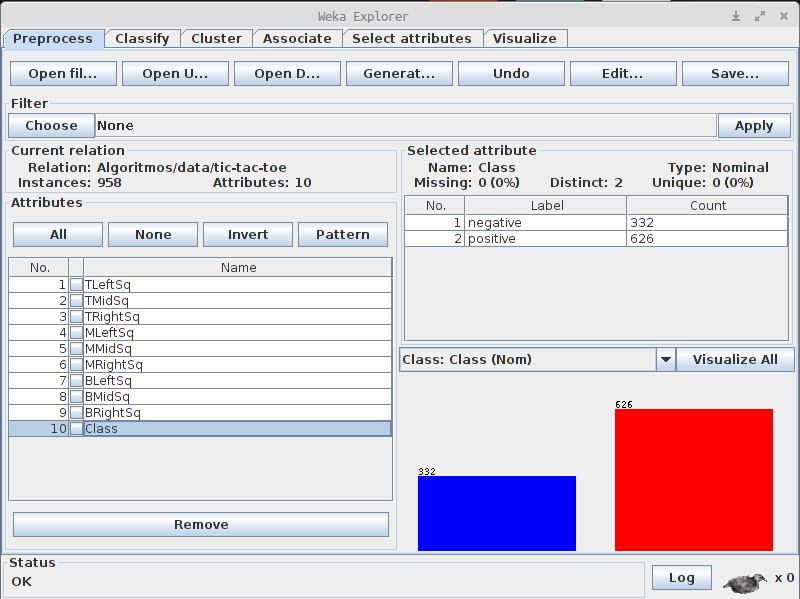
\includegraphics[scale=0.5]{img/Tic-tac-toe_APriori.png}
\end{center}

Nuestro clasificador a Priori contaba: { negative = 254, positive = 464} . ¿A qué se debe esta diferencia? Nuestro clasificador a Priori ignora al leer el fichero todas las filas que contengan alguna "?". En cambio Weka, sólo ignora estas filas cuando necesita utilizar ese dato. Para clasificar a Priori no necesitamos saber la media exacta del atributo TLeftSq por ejemplo. Si en ese atributo hay alguna "?", Weka elimina la fila al necesitar el valor, nuestra implementación al cargar el fichero.
Independientemente de esta diferencia de implementación (que podría ser significativa) observamos que el error cometido por Weka es 34.6555\% y por nuestra implementación 35.3760 \%. 


\paragraph{Una vez comentado esto, procedemos a clasificar con NaiveBayes los datos:}
\subsection{Crx}

Incluimos una captura de pantalla de Weka, y a continuación comentamos los resultados:

\begin{center}
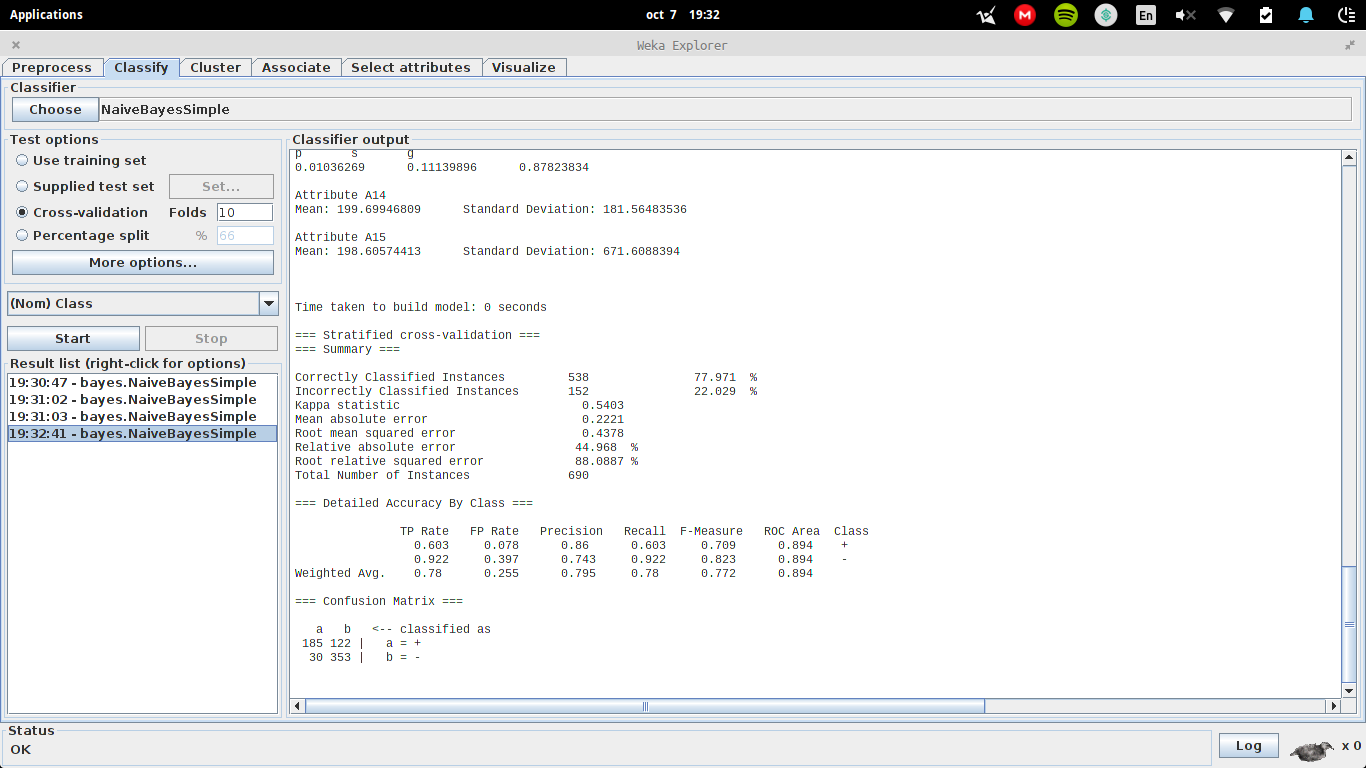
\includegraphics[scale=0.3]{img/crx_NBSimple.png}
\end{center}


Observamos que ha clasificado mal un 22\% de las muestras. Actualmente no podemos comparar este clasficador por el implementado en la Práctica 1 ya que no llegamos a implementarlo. 

\paragraph{Matriz de confusión:} Comentamos la matriz de confusión, que es una manera de representar el error muy visual:

\begin{center}
\begin{tabular}{c|cc}
Clasificado como $\to$ & a & b \\\hline
siendo $a = +$ & 185 & 122 \\
siendo $b = -$ & 30 & 353
\end{tabular}
\end{center}


Es curioso que, siendo una muestra de clase "-", es clasificada correctamente en un porcentaje mucho mayor (92\%) que siendo "+" (60\%). Concluimos que es más fácil reconocer los "-" que los "+".

\subsection{Tic-tac-toe}

Incluimos una captura de pantalla de Weka, y a continuación comentamos los resultados:

\begin{center}
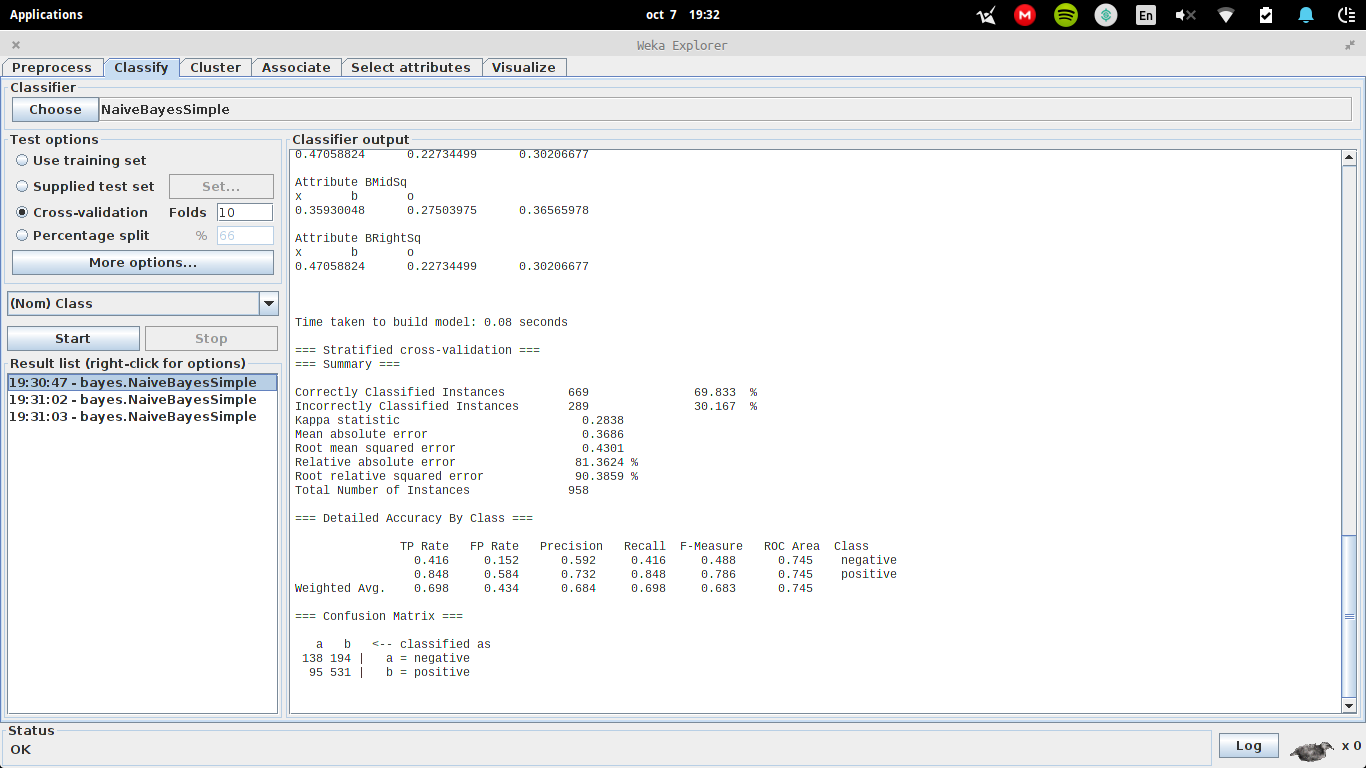
\includegraphics[scale=0.3]{img/Tic-tac-toe_NBSimple.png}
\end{center}

Observamos que ha clasificado mal un 30\% de las muestras. Este porcentaje es demasiado elevado como para poder confiar en este clasificador. Esperamos que con los algoritmos que vayamos aprendiendo a lo largo del curso se pueda clasificar con un porcentaje menor este conjunto de datos. Actualmente no podemos comparar este clasficador por el implementado en la Práctica 1 ya que no llegamos a implementarlo.  

\paragraph{Matriz de confusión:} Comentamos la matriz de confusión, que es una manera muy visual de representar el error:

\begin{center}
\begin{tabular}{c|cc}
Clasificado como $\to$ & a & b \\\hline
siendo $a = neg$ & 138 & 194 \\
siendo $b = pos$ & 95 & 531
\end{tabular}
\end{center}
En este caso, observamos que la tasa de error de dar como "positive" un elemento "negative" es superior al 50\% (58\%), en cambio dar como "negative" un elemento "positive" es del 15\%, un porcentaje mucho más aceptable.

\section{Vecinos próximos}


\section{Regresión logística}


\section{Profundizando sobre vecinos próximos}



\end{document}
